
\section{Evaluation}
In this section, we evaluate the uniRDMA prototype on the physical RDMA platform. In addition to the basic network performance, such as throughput and latency, it also includes real-wprd RDMA applications. We expect to answer the following questions:
(1)Can uniRDMA's network performance in container and virtual machine environments be close to native RDMA?
(2)Does uniRDMA have high scalability in both large-scale container and virtual machine cluster environments?
(3)Can uniRDMA be adapted to the real RDMA application environment in containers and virtual machines?
	
\subsection{Experiment Methodology}
All experiments are carried out on two servers. The settings mainly include three parts: host server, container and virtual machine. The detailed settings are shown in Table~\ref{tab:exp-env}:

\begin{table}
	\newcommand{\tabincell}[2]{\begin{tabular}{@{}#1@{}}#2\end{tabular}}
	\caption{Experiment Environments}
	\label{tab:exp-env}
	\begin{tabular}{c|c|l} 
		\hline 
		% \multicolumn{2}{c|}{Flag}
		\multicolumn{2}{c|}{Parameters} & Settings\\ \hline
		\multirow{7}{*}{Server} 
		& CPU &  \tabincell{l}{Four Intel Xeon E7-4850 \\  v4 16-core CPUs } \\ \cline{2-3}
		& Memory & 1 TiB DDR4/DDR3 \\  \cline{2-3}
		& Kernel & CentOS 7.4.1708 \\  \cline{2-3}
		& Physical RNIC & \tabincell{l}{Mellanox ConnectX-3 \\ 56 Gb/s}\\  \cline{2-3}
		& RDMA Driver &	\tabincell{l}{Mellanox OFED \\4.4-2.0.7.0} \\  \cline{2-3}
		& Hypervisor & QEMU 5.1.50 \\ \cline{2-3}
		& Container Engine & Docker 18.06.1-ce \\ \hline
		\multirow{3}{*}{VM} 
		& CPU & 16 cores \\  \cline{2-3}
		& Memory & 64 GB \\  \cline{2-3}
		& Kernel & CentOS 7.4.1708 \\  \hline
		\multirow{3}{*}{Container} 
	 	& CPU & 16 cores \\  \cline{2-3}
	 	& Memory & 64 GB \\  \cline{2-3}
	 	& Image & CentOS 7.4.1708\\ \hline 
	\end{tabular}
\end{table}

The RNIC used by the server is Mellanox ConnectX-3 56 Gb/sec, which performs RDMA communication under Infiniband. The operating system of servers is CentOS 7.4.1708, and the Linux kernel version is 3.10.0-693.el7.x86\_64. The RDMA driver installed on the host server is Mellanox OFED 4.4-2.0.7.0~\cite{mlnx-ofed}, which adapts to the RNIC and host operating system. To get consistence, virtual machines and containers are built based on the same OS images as host. All virtual machines are based on QEMU(5.1.50)~\cite{qemu} enabled with KVM~\cite{kvm} and the container engines are Docker(18.06.1-ce)~\cite{docker}. In addition, the entire uniRDMA framework is compiled with GCC/G++ 4.8.5, and the O3 compilation optimization level is selected. 

\subsection{Basic benchmark}
Throughput and latency are the key target of network performance. RDMA supports two different data transmission modes: unilateral and bilateral. Due to the difference performance between thems, we evaluate them respectively.

Based on the RDMA benchmark test tool Mellanox perftest, we evaluated the throughput and latency of uniRDMA, native RDMA, hardware virtualization SR-IOV, and software virtualization FreeFlow in virtual machines or containers. For bilateral operations (Send and Recv), we use the ``ib\_send\_bw'' and ``ib\_send\_lat'' commands; for two unilateral operations (Write and Read), with Write as the representative, we use the ``ib\_write\_bw'' and ``ib\_write\_lat'' commands. The specific process is: after the RDMA connection is established between the client and the server, the bytes of  transmitted message each time will be increased from 4B to 1MB, the data will be iteratively transmited 1000 times with each message size, and finally the average throughput and latency are calucated.

(1)Throughput: The results of bilateral operation are shown in Figure~\ref{fig:send-bw}, and the one of unilateral operation are shown in Figure~\ref{fig:write-bw}. Whether uniRDMA is in a virtual machine or in a container scenario, the throughput of its bilateral and unilateral operations is slimilar as SR-IOV and close to native RDMA.

Compared with FreeFlow, when the message is small, the throughput of uniRDMA has reached 4-6 times that of FreeFlow. Because FreeFlow forwards all data commands to the software virtualization layer for processing. Therefore, the forward latency gradually accumulates and decrease the throughput significantly. However, uniRDMA maps all RDMA resources to execute data commands in the user space of the container or virtual machine. Therefore, there is no latency for  commands forwarding in data path.

\begin{figure}[!ht]
	\centering
	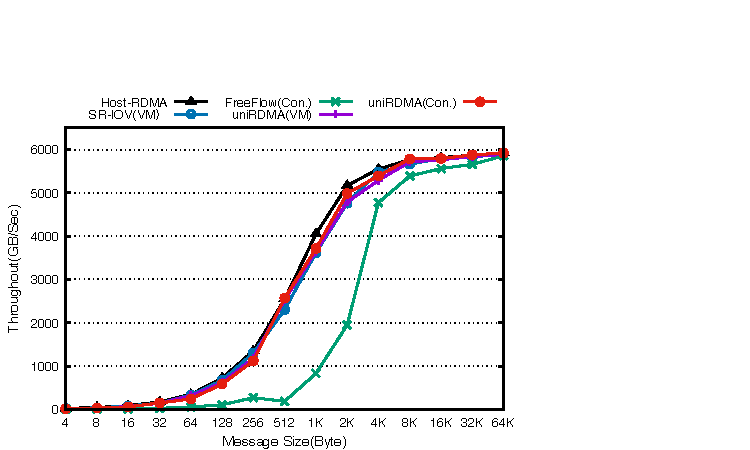
\includegraphics[width=1.0\linewidth]{images/send-bw.pdf}
	\caption{The Throughout of RDMA Send and Recv}
	\label{fig:send-bw}
\end{figure}

\begin{figure}[!ht]
	\centering
	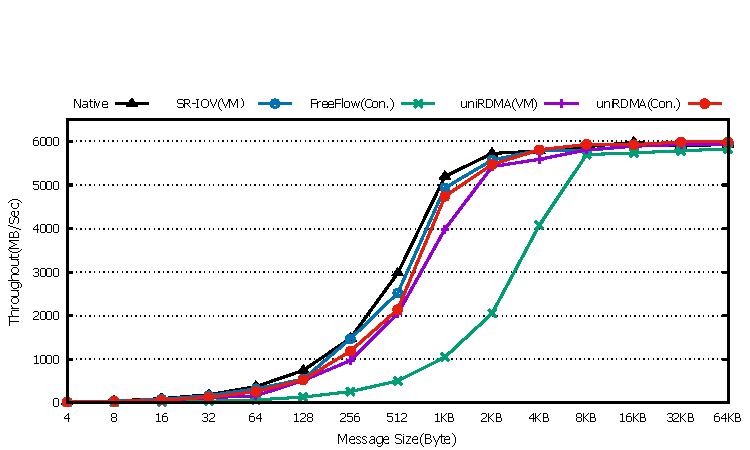
\includegraphics[width=1.0\linewidth]{images/write-bw.pdf}
	\caption{The Throughout of RDMA Write}
	\label{fig:write-bw}
\end{figure}

When the message gradually increases, such as reaching 64KB, the throughput of each framework tends to be consistent. The reason is that the bandwidth is saturated, and the delay overhead of FreeFlow has been covered by waiting delay in RNIC.

(2)latency: The results of bilateral operation are shown in Figure~\ref{fig:send-lat}, and the one of unilateral operation are shown in Figure~\ref{fig:write-lat}. Whether uniRDMA is in a virtual machine or in a container scenario, the latency of its bilateral and unilateral operations is slimilar as SR-IOV and close to native RDMA.

Compared with FreeFlow, when the message is small, the latency of uniRDMA has reached 40\%~60\%  of FreeFlow beacause of FreeFlow's forwarding latency. Also, when the message gradually increases, such as reaching 64KB, the latency of each framework tends to be consistent. Beacause the main latency has been caused by RNIC data processing.

\begin{figure}[!ht]
	\centering
	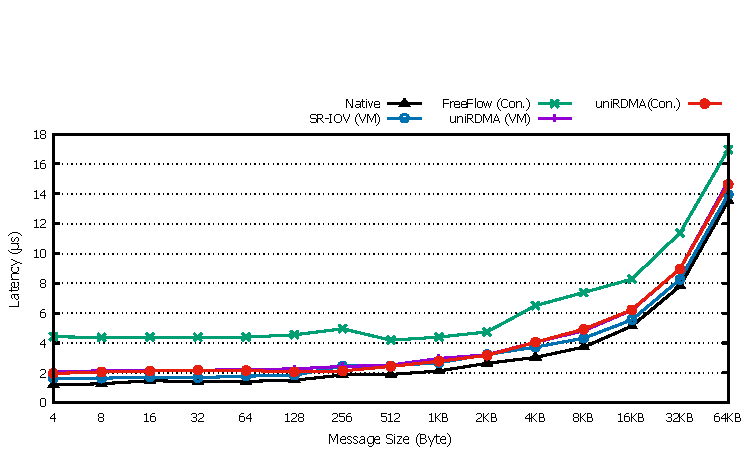
\includegraphics[width=1.0\linewidth]{images/send-lat.pdf}
	\caption{The Latency of RDMA Send and Recv}
	\label{fig:send-lat}
\end{figure}

\begin{figure}[!ht]
	\centering
	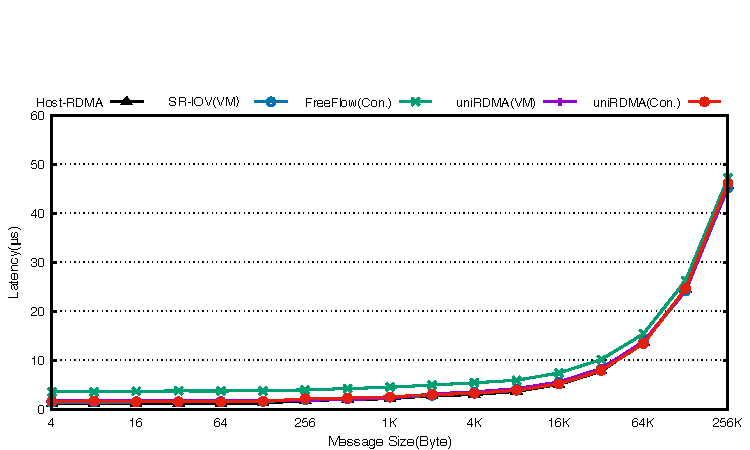
\includegraphics[width=1.0\linewidth]{images/write-lat.pdf}
	\caption{The Latenct of RDMA Write}
	\label{fig:write-lat}
\end{figure}
(3)Scabality: 
Scalability is a challenge when RDMA virtualization in large-scale virtual clusters. To evaluate uniRDMA's scalabilitu, for 2, 4, 8, 16, 32, 64, and 128 pairs of virtual instances, a random number of virtual instances are selected to execute ``ib\_write\_bw'' command with 128KB message. Moreover, there are full virtual machines, full containers and hybrid virtual instances(50\% virtual machine and 50\% containers) when evaluating. Finally, the average throughput between virtual instance pairs is shown in Figure~\ref{fig:scabality}.

\begin{figure}[!ht]
	\centering
	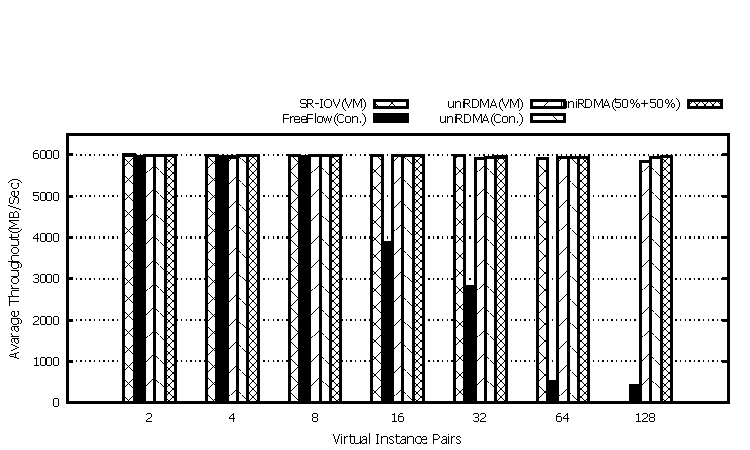
\includegraphics[width=1.0\linewidth]{images/scabality.pdf}
	\caption{The Scabality}
	\label{fig:scabality}
\end{figure}

From Figure~\ref{fig:scabality}, for all virtual environments, uniRDMA has good scalability and still maintains high performance. In contrast, the throughput of FreeFlow is down to only 10\% throughput compared to the peak. Because uniRDMA data commands do not need to be forwarded to the software virtualization layer for processing, the virtualization overhead does not increase due to the expansion of virtual instances. Constractly, whhen FreeFlow runs RDMA commands at the same time in a large-scale container, it is forwarded to the same RDMA context in virtual layer. When calling the QP queue or registered memory region in virtual layer, there is the overhead of lock mutual exclusion. Therefore, FreeFlow suffers from a drastic drop in performance in large-scale container scenarios.

In addition, as shown in Figure~\ref{fig:scabality}, both uniRDMA and FreeFlow can support communication between 128 pairs of virtual instances. However, the maximum number of VFs of the Mellanox ConnectX-3 network card is only 126, so 128 pairs of virtual instances are not supported. This shows that uniRDMA has higher scalability than SR-IOV. Because VFs are statically allocated in SR-IOV and each VF is exclusively occupied by the virtual machine; while uniRDMA improves the utilization of VF through  dynamic device pool and flexible mapping mechanism in virtual layer.

\subsection{Real-world Applications}

The worth of RDMA is mainly about its optimized performance in real-world applications. RDMA virtualization needs to maintain the performance close to native RDMA. Therefore, we evaluate uniRDMA and other frameworks in different RDMA applications, such as high-performance computing benchmark Graph-500 and data processing framework Spark-RDMA.

(1)Graph-500: For high-performance computing, Graph-500 is a benchmark framework used to test the performance of the Message Passing Interface (MPI) [42]. Based on the constructed graph structure, users test the performance of breadth-first search (BFS) and single source shortest path (SSSP). The performance index is the number of edges traversed per second (traversed edges). per second, TEPS), the larger the value, the better the performance.

In this paper, the node scale of the computational graph in Graph-500 is set to 26, and the ratio of edges to points is set to the default parameter of 16. The constructed graph has a total of 2\^25 vertices, with 2\^29 edges, the entire graph occupies approximately around 16GB. When testing BFS and SSP, 16 MPI processes are scattered and executed on two nodes in turn, and the average value is taken according to the results of 12 tests. The data obtained is shown in Table Figure~\ref{fig:graph-500} (because there are core dump problems when using FreeFlow for Graph-500, the corresponding data is lacking).

As shown in Figure~\ref{fig:graph-500},  the performance of uniRDMA is close to native RDMA. Beacause uniRDMA bypasses the kernel and virtualization layer in the data path, and there is no forwarding latency.

\begin{figure}[!ht]
	\centering
	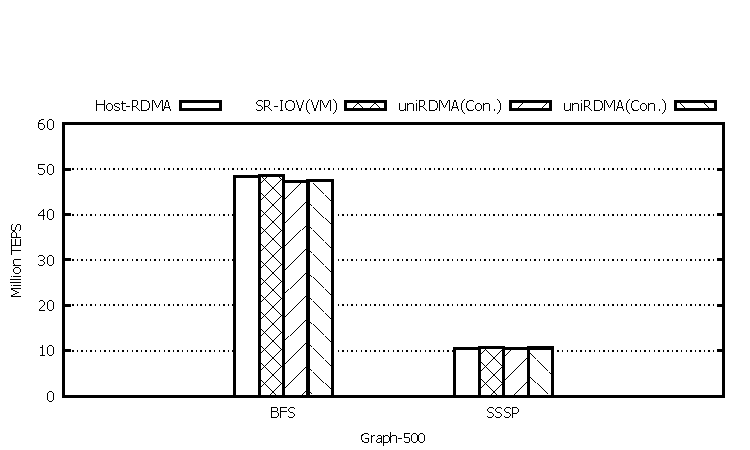
\includegraphics[width=1.0\linewidth]{images/graph-500.pdf}
	\caption{The Performance of Graph-500}
	\label{fig:graph-500}
\end{figure}

(2)Spark-RDMA: It is a classical big data processing framework for distributed computing. Based on Spark-RDMA (v0.9.5), we run two tasks: GroupBy and SortBy. For each task, two Spark processes are run on two servers. At the same time, the number of cores used is limited to 8 and the memory is 32GB. There are 8 mappers and 8 reducers for 262144 key-value pairs of 2KB. At last, we run 12 times for each task to get the avarage execution time.